\titleformat{\chapter}[display]
{\normalfont\Large\BNazboldEGT\centering}
{\vspace*{8cm}{\textbf{‎فصل سوم} }}{5pt}{\Large}
\chapter{\textbf{روش پیشنهادی}}\label{sec3}
\thispagestyle{empty}
\newpage

\begin{figure}
	\centering
	\scriptsize
	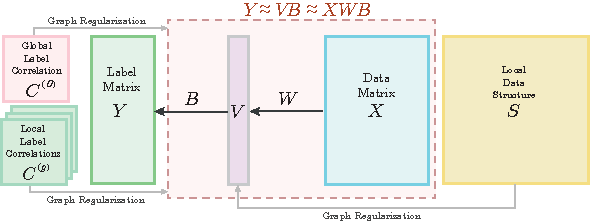
\includegraphics[width=12cm,height=5cm]{../figures/Fig1_2.pdf}
	\caption{شمای کلی روش پیشنهادی \lr{(MLFS-GLOCAL)}}
	\label{fig:1}
\end{figure}

\section{مقدمه} \label{sec31}

در این فصل، انتخاب ویژگی چندبرچسبه با استفاده از همبستگی سراسری و محلی برچسب‌ها )‎\lr{MLFS-GLOCAL‎}) معرفی می‌شود و از همبستگی برچسب‌های سراسری و محلی برای انتخاب ویژگی‌های مرتبط و غیرتکراری استفاده می‌کند. موفقیت مدل ارائه شده به چهار عامل اصلی بستگی دارد:
(1) برای ارائه یک بازنمایی برچسب-ویژگی بهینه‌تر، ساختار رتبه‌پایین را از ماتریس‌های برچسب و ویژگی استخراج می‌شود. در این فضای کاهش یافته، یک همبستگی ضمنی بین برچسب‌ها وجود دارد (بخش \ref{lowrank}‎.(
(2) جریمه‌ای\LTRfootnote{Penalty } اعمال می‌شود که همواری نگاشت محلی را در فضای نهان مشترک حفظ می‌کند (بخش \ref{LS}).
(3) با استفاده از اطلاعات همبستگی‌های سراسری و محلی برچسب، از ماتریس برچسب بصورت بهینه‌تر استفاده کرد (بخش \ref{GLOCAL}).
(4) مسئله، با ترکیب موارد فوق به یک مدل یادگیری مشترک متصل تبدیل می‌شود و از یک رویکرد کمینه‌سازی متناوب مؤثر برای بهینه‌سازی استفاده می‌کند
(بخش \ref{OPT}.(‎
شکل ‎\ref{fig:1} نمایش شماتیک از مدل ‎\lr{MLFS-GLOCAL} را ارائه می‌دهد.
\section{فضای نهان مشترک}\label{lowrank}
ماتریس ویژگی به‌صورت $\boldmath{X} \in \mathbb{R}^{n \times d}$ تعریف می‌شود و ماتریس برچسب به‌صورت $\boldmath{Y} = \{\boldmath{y}_1, {\dots}, \boldmath{y}_l\} \subseteq \{0,1\} \in \mathbb{R}^{n \times l}$ تعریف می‌شود که
${Y}_{i,j}=1$
اگر نمونه $i$-ام، برچسب $j$-ام را داشته باشد، در غیر این‌صورت  ${Y}_{ij}=0$. در مسائل داده‌های چندبرچسبه، برچسب‌ها با یکدیگر مرتبط هستند، از این رو می‌توان از رتبه‌پایین این ماتریس استفاده کرد. محتویات ماتریس خلوت $\boldmath{Y}$، دارای مقادیر دودویی و ابعاد بالا می‌باشد، بنابراین یادگیری براساس این ماتریس مشکل است. لذا اندازه ماتریس کم‌بُعد $\boldmath{Y}$ بصورت $‎‎‎k<\text{‎\lr{min}‎}(n,l)$ خواهد بود،
از این رو، ماتریس برچسب را به دو ماتریس کوچکتر به‌صورت زیر تجزیه می‌کنیم:
\begin{align}
	\boldmath{Y}\simeq\boldmath{VB}
\end{align}
که $\boldmath{V} \in \mathbb{R}^{n \times k} $ و $\boldmath{B} \in \mathbb{R}^{k \times l}$.‎


$\boldmath{V}$
ماتریس نهان برچسب‌ها است که فشرده‌تر\LTRfootnote{Compact} و از نظر معنایی انتزاعی‌تر از ماتریس برچسب‌های اصلی هستند.
$\boldmath{B}$
نشان می‌دهد که چگونه برچسب‌های اصلی با برچسب‌های نهفته مرتبط هستند. اطلاعات مهم ماتریس برچسب اصلی $\boldmath{Y}$ در ماتریس کم‌بُعد $\boldmath{V}$ کدگذاری شده است که همچنین داده‌های نامطلوب ماتریس برچسب را کاهش می‌دهد. ماتریس های $\boldmath{V}$ و $\boldmath{B}$ با به حداقل رساندن خطای بازنمایی برچسب $\lVert\boldmath{Y} - \boldmath{VB}\rVert^2_F$ بدست می‌آید. بازنمایی برچسب نهان، با $\boldmath{V}$ نشان داده شده است، یک ماتریس با ابعاد کم و با مقدار حقیقی که حاوی اطلاعات متراکم می‌باشد. بنابراین یادگیری نگاشت پیوسته از فضای ویژگی به فضای برچسب نهفته نسبتاً آسان‌تر از فضای برچسب اصلی است\cite{zhu2017multi}.
یک فرض مهم در رابطه‌ی همبستگی بین ویژگی‌ها و برچسب‌ها این می‌باشد که ویژگی‌های مشابه، برچسب‌های مشابهی دارند. در نتیجه، اطلاعات مشترک بین فضای ویژگی و فضای برچسب باید سازگار باشد. ما درنظر می‌گیریم $\boldmath{V}$ یک ماتریس مشترک بین ماتریس ویژگی و ماتریس برچسب باشد. ماتریس $\boldmath{W} \in \mathbb{R}^{d \times k}$ بروزرسانی می‌شود جهت نگاشت نمونه‌ها به فضای نهان. با کاهش خطای تابع بازنمایی ویژگی $\lVert\boldmath{V} - \boldmath{XW}\rVert^2_F$، ماتریس وزن ویژگی $\boldmath{W}$ آموخته خواهد شد و با ادغام بازنمایی برچسب و خطای بازنمایی ویژگی در یک چارچوب ماتریس نامنفی \cite{lee1999learning}، فضای نهان مشترک را از طریق تابع زیر بدست می‌آوریم:
\begin{align}
	\min_{\boldmath{V},\boldmath{B},\boldmath{W}}&\lVert\boldmath{Y}-\boldmath{V}\boldmath{B}\rVert^2_F+\lVert\boldmath{V}-\boldmath{X}\boldmath{W}\rVert^2_F,\quad{\text{\lr{s.t.}}\quad}\boldmath{{V,B,W}}\geq 0
\end{align}
\section{حفظ ساختار محلی}\label{LS}
در بسیاری از کاربرد‌های یادگیری ماشین، فضای ویژگی می‌تواند دارای ابعاد بالا همراه با نویز باشد، که استخراج اطلاعات معنی‌دار از داده‌ها را به چالش می‌کشاند. یکی از روش‌های رایج برای استخراج اطلاعات مفید، تبدیل فضای ویژگی اصلی به فضای نهان با ابعاد پایین‌تر است، جایی که ساختار زیربنایی داده‌ها را می‌توان راحت‌تر بدست ‌آورد. با این حال، بازنمایی داده‌ها در فضایی با ابعاد پایین‌تر می‌تواند منجر به از دست رفتن اطلاعات\LTRfootnote{Loss of information} شود و ممکن است روابط پیچیده بین ویژگی‌ها را به درستی نشان ندهد، از این رو از  یک منظم‌ساز گراف \cite{cai2010graph} برای ارائه یک ماتریس مناسب $\boldmath{V}$ که انسجام بین فضای ویژگی اولیه و فضای ساختار نهان را تضمین ‌کند استفاده می‌کنیم. با توجه به اصل اساسی این قاعده‌بندی، اگر دو نمونه در فضای ماتریس ویژگی $\boldmath{X}$ با یکدیگر همبستگی داشته باشند، در فضای ساختار نهان نیز هر دو نمونه $\boldmath{v}_i$ و $\boldmath{v}_j$ با یکدیگر همبستگی خواهند داشت. به‌طور خاص، ما از یک منظم‌ساز گراف برای تشویق حفظ ساختار محلی در فضای نهان استفاده می‌کنیم، و اطمینان حاصل می‌کنیم که متغیرهای نهفته به‌طور دقیق ساختار ویژگی‌های اصلی را منعکس می‌کنند. فرمول منظم‌ساز گراف را می‌توان به‌صورت زیر بیان کرد:
\begin{align} \label{eq:mfold}
	\min_{\boldmath{V}}&\frac{1}{2}\sum_{i=1}^n\sum_{j=1}^n\lVert\boldmath{v}_i-\boldmath{v}_j\rVert^2S_{i,j}\nonumber\\
	&=\frac{1}{2}\sum_{i=1}^n\sum_{j=1}^n(\boldmath{v}_i^\top\boldmath{v}_iS_{i,j}-2\boldmath{v}_i^\top\boldmath{v}_jS_{i,j}+\boldmath{v}_j^\top\boldmath{v}_jS_{i,j})\nonumber\\
	&=\frac{1}{2}\sum_{i=1}^n\sum_{j=1}^n(2\boldmath{v}_i^\top\boldmath{v}_iS_{i,j}-2\boldmath{v}_i^\top\boldmath{v}_jS_{i,j})\nonumber\\
	&=\sum_{i=1}^n\boldmath{v}_i^\top\boldmath{v}_iD_{i,i}-\sum_{i=1}^n\sum_{j=1}^n\boldmath{v}_i^\top\boldmath{v}_jS_{i,j}\nonumber\\
	&=\mathrm{Tr}(\boldmath{V}^\top\boldmath{DV})-\mathrm{Tr}(\boldmath{V}^\top\boldmath{SV})=\mathrm{Tr}(\boldmath{V}^\top \boldmath{LV}),
\end{align}
که
$\boldmath{D}$ ماتریس قطری\LTRfootnote{Diagonal} و $\boldmath{S}$ ماتریس همبستگی متقارن\LTRfootnote{Symmetric} است. $\boldmath{L} = \boldmath{D} - \boldmath{S}$ ماتریس لاپلاسین گراف می‌باشد. با ادغام عبارات فوق در مدل، تابع زیر را بدست می‌آوریم:

\begin{align}\label{eq:m-mfold}
	\min_{\boldmath{V},\boldmath{B},\boldmath{W}}&\lVert\boldmath{Y}-\boldmath{V}\boldmath{B}\rVert^2_F+\lVert\boldmath{V}-\boldmath{X}\boldmath{W}\rVert^2_F +\lambda_1{\mathrm{Tr}\boldmath{({V}^\top{LV})}}
	,\nonumber \\
	&{\text{\lr{s.t.}}}\boldmath{V},\boldmath{B},\boldmath{W}\geq 0
\end{align}
که 
$\lambda_1$
پارامتر حفظ ساختار محلی است.
\section{همبستگی برچسب سراسری و محلی}\label{GLOCAL}
برای استفاده مؤثر از اطلاعات برچسب‌ها، باید از همبستگی‌های برچسب استفاده شود. در این روش، مدل پیشنهادی را با استفاده از همبستگی برچسب مرتبه‌بالا منظم می‌کنیم. در این راستا باید به همزیستی\LTRfootnote{Coexistence} همبستگی‌های سراسری و محلی برچسب اشاره کرد. برای ترکیب هر دوی آن‌ها، منظم‌ساز خمینه برچسب‌ها را در این قسمت معرفی می‌کنیم. مفهوم منظم‌ساز خمینه سراسری برچسب‌ ‌از منظم‌ساز خمینه سطح نمونه \eqref{eq:mfold} مشتق شده است. به‌طور دقیق‌تر اگر دو برچسب دارای همبستگی بالایی باشند، خروجی‌های طبقه‌بند مربوطه آن‌ها نیز باید شباهت داشته باشند و برعکس، برچسب‌هایی که دارای همبستگی کمتری هستند باید خروجی‌های طبقه‌بند آن‌ها شباهت کمتری داشته باشند. به عبارت دیگر، همبستگی‌های برچسب منجر به خروجی‌های طبقه‌بند مشابه می‌شود. در این تحقیق از شباهت کسینوس\LTRfootnote{Cosine Similarity} برای تعیین کمیت همبستگی سراسری برچسب استفاده می‌شود $\boldmath{C} \in\mathbb{R}^{l \times l}$، که به‌صورت زیر محاسبه می‌شود: 
\begin{align}\label{eq:gloCor}	
	{{{C}_{ij}=\frac{\boldmath{y}^\top_{i}{\boldmath{y}_{j}}}{{\lVert{\boldmath{y}_i}\lVert} \lVert{\boldmath{y}_{j}}\lVert}}}
\end{align}
که
$\boldmath{y}_i$ 
, 
$\boldmath{y}_j$
به مفهوم $i$-ام و $j$-ام بردار برچسب برای همه‌ی نمونه‌ها می‌باشد.‎\\
در\eqref{eq:m-mfold}، برچسب پیش‌بینی شده برای $\boldmath{x}$ به‌صورت $f(\boldmath{x})$ است، که $f(\boldmath{x}) = \boldmath{x}\boldmath{WB}$. 
$\boldmath{f} = \{{f}_1, {\dots}, {f}_l\}$
که $\boldmath{f}_j(\boldmath{x})$ یعنی $j$-ام برچسب برای نمونه $\boldmath{x}$ پیش‌بینی شده است. در نهایت پیش‌بینی برای همه‌ی ${n}$ نمونه در ماتریس پیش‌بینی $\boldmath{F}\in\mathbb{R}^{n \times l}$ ذخیره می‌شود،‌ $\boldmath{F}= \{f({\boldmath{x}}_1),{\dots},f({\boldmath{x}}_n)\}^\top = \boldmath{XWB}$ شامل محتویات پیش‌بینی شده برای $i$-ام برچسب $\boldmath{f}_i$، اگر برچسب ${i}$-ام و ${j}$-ام شبیه باشند باید بردار پیش‌بینی شده
$\boldmath{f}_j$ و $\boldmath{f}_i$
این دو برچسب نیز شبیه باشند و برعکس. تعریف منظم‌ساز خمینه ‌سراسری برچسب شبیه تعریف منظم‌ساز خمینه نمونه \eqref{eq:mfold} است و به‌صورت زیر تعریف می‌شود:
\begin{align}\label{eq:glomfold}
	\min_{\boldmath{F}}&\frac{1}{2}\sum_{i=1}^l\sum_{j=1}^l\lVert\boldmath{f}_i-\boldmath{f}_j\rVert^2C_{i,j}=\nonumber\\
	&\mathrm{Tr}(\boldmath{FA}\boldmath{F}^\top)-\mathrm{Tr}(\boldmath{FC}\boldmath{F}^\top)=\mathrm{Tr}(\boldmath{FP}\boldmath{F}^\top),\nonumber\\
\end{align}
$\boldmath{A}$ ماتریس قطری و به‌صورت ${A}_{ii}=\sum_{j=1}^l {C}_{ij}$ تعریف می‌شود. 
با کمینه‌سازی کردن \eqref{eq:glomfold}، خطای $\lVert\boldmath{f}_i-\boldmath{f}_j\rVert^2 $ کم خواهد بود. منظم‌ساز خمینه در \eqref{eq:glomfold} به‌صورت $\mathrm{Tr}(\boldmath{FPF}^\top)$، که $\boldmath{P} = \boldmath{A}-\boldmath{C}$ ماتریس لاپلاسین ‌است. $\boldmath{F}=\boldmath{XWB}$ برچسب‌های پیش‌بینی شده برای ویژگی‌ها می‌باشد. از آنجایی که همبستگی‌های برچسب می‌تواند در نواحی مختلف محلی متفاوت باشد، برای استخراج این همبستگی‌ها از منظم‌ساز خمینه محلی استفاده می‌کنیم. فرض می‌کنیم که مجموعه‌داده\LTRfootnote{Dataset} $\boldmath{X}$ به ${g}$ گروه $\{\boldmath{X}_1,{\dots},\boldmath{X}_g\}$ تقسیم می‌شود، ماتریس $\boldmath{X}_m \in \mathbb{R}^{n_m \times d}$ نمونه دارد. با استفاده از خوشه‌بندی، مانند شبکه‌ها\LTRfootnote{Networks} و مسیرهای ژنی\LTRfootnote{Pathways} \cite{chuang2007network,subramanian2005gene} در کاربردهای بیوانفورماتیک\LTRfootnote{Bioinformatics}، امکان دستیابی به این پارتیشن‌بندی وجود دارد. فرض  $\boldmath{C}_m \in \mathbb{R}^{{l} \times {l}}$ ماتریس همبستگی برچسب محلی یک گروه ${m}$ است. و $\boldmath{Y}_m$ زیر ماتریس برچسب در $\boldmath{Y}$ متناظر با $\boldmath{X}_m$ است. مانند \eqref{eq:gloCor}، ما همبستگی‌های برچسب محلی را به‌صورت زیر محاسبه می‌کنیم:

\begin{align}\label{eq:llc}	
	{{{C}^{(m)}_{i,j}}=
		\frac
		{{\boldmath{y}^{(m)}_{i}}^\top\boldmath{y}^{(m)}_{j}}
		{{\lVert{\boldmath{y}^{(m)}_{i}}\lVert}\lVert{\boldmath{y}^{(m)}_{j}}\lVert}}, \; m \in  \{1,{\dots},{g}\}
\end{align}
مشابه همبستگی برچسب سراسری \eqref{eq:glomfold}، اگر دو برچسب با همدیگر همبستگی داشته باشند باید بردار ‎‎پیش‌بینی شده‎ طبقه‌بند نیز شبیه باشند:
\begin{align}\label{eq:loclmfold}
	\min_{\boldmath{F}}&\sum_{m=1}^{g}\frac{n_m}{n}\sum_{i=1}^{l}\sum_{j=1}^{l} \lVert{\boldmath{f}^{(m)}_i}-{\boldmath{f}^{(m)}_j}\rVert^2 {C^{(m)}_{i,j}}\nonumber \\
	&=\sum_{m=1}^{g} \frac{n_m}{n}[\mathrm{Tr}(\boldmath{F}_m\boldmath{A}_m\boldmath{F}_m^\top) - \mathrm{Tr}(\boldmath{F}_m \boldmath{C}_m \boldmath{F}_m^\top)]\nonumber \\
	&= \sum_{m=1}^{g}\frac{n_m}{n}\mathrm{Tr}(\boldmath{F}_m \boldmath{P}_m \boldmath{F}_m^\top)
\end{align}
که $\boldmath{F}_m = \boldmath{X}_m\boldmath{WB}$ ماتریس خروجی طبقه‌بند برای گروه $m$ است و $\boldmath{P}_m$ ماتریس لاپلاسین $\boldmath{C}_m$ است. برای پوشش عدم تعادل\LTRfootnote{Imbalance} خوشه، منظم‌ساز همبستگی محلی برچسب را با ضریب ${n_m}/{n}$  نرمال می‌کنیم.
پس از افزودن منظم‌سازهای خمینه سراسری \eqref{eq:glomfold} و محلی  \eqref{eq:loclmfold} به تابع \eqref{eq:m-mfold}، فرمول زیر بدست می‌آید:
\begin{align}
	&\min_{\boldmath{V},\boldmath{B},\boldmath{W}}\lVert\boldmath{Y}-\boldmath{V}\boldmath{B}\rVert^2_F+\lVert\boldmath{V}-\boldmath{X}\boldmath{W}\rVert^2_F+\lambda_1{\mathrm{Tr}\boldmath{({V}^\top{LV})}}
	\nonumber \\&+\lambda_2[\mathrm{Tr}(\boldmath{FP}\boldmath{F}^\top) 
	+ \sum_{m=1}^{g}\frac{n_m}{n}\mathrm{Tr}(\boldmath{F}_m\boldmath{P}_m\boldmath{F}^\top_m) ],
	\quad{\text{\lr{s.t.}}\quad}\boldmath{V},\boldmath{B},\boldmath{W}\geq 0 
\end{align}
که $\lambda_2$ نشان دهنده تأثیر همبستگی برچسب سراسری و محلی برای تابع هدف است. در نهایت، تابع ما از نُرم $\ell_{2,1} $، که برای انتخاب ویژگی است استفاده می‌کند. در نتیجه تابع نهایی به‌صورت زیر تنظیم می‌شود: 
\begin{align}\label{eq:BeOpt}
	&\min_{\boldmath{V},\boldmath{B},\boldmath{W}}\lVert\boldmath{Y}-\boldmath{V}\boldmath{B}\rVert^2_F+\lVert\boldmath{V}-\boldmath{X}\boldmath{W}\rVert^2_F+\lambda_1{\mathrm{Tr}\boldmath{({V}^\top{LV})}} \nonumber \\ 
	& +\lambda_2[\mathrm{Tr}(\boldmath{FP}\boldmath{F}^\top)+\sum_{m=1}^{g}\frac{n_m}{n}\mathrm{Tr}(\boldmath{F}_m\boldmath{P}_m\boldmath{F}^\top_m) ]+ \lambda_3\lVert\boldmath{W}\rVert_{2,1},\nonumber \\ &{\text{\lr{s.t.}}}\boldmath{V},\boldmath{B},\boldmath{W}\geq 0 \nonumber \\
\end{align}
با استفاده از نُرم $\ell_{2,1} $ بر روی سطر ماتریس $\boldmath{W}$ خلوتی اعمال می‌کنیم و منظم‌ساز خلوتی تابع هدف نیز توسط پارامتر $\lambda_3$ کنترل می‌شود.

\section{بهینه‌سازی}\label{OPT} 
تابع \eqref{eq:BeOpt} شامل عبارت منظم‌ساز نُرم $\ell_{2,1} $ است. از آنجا که این تابع هموار نیست، همچنین وقتی متغیرهای $\boldmath{V}$، $\boldmath{B}$ و $\boldmath{W}$ به‌صورت ترکیبی درنظر گرفته می‌شوند، غیرمحدب\LTRfootnote{Non-convex} می‌شود. به‌عبارت دیگر، ماتریس هسین\LTRfootnote{Hessian matrix} که از مشتقات جزئی تابع هدف در درجه‌دوم بدست می‌آید، ماتریسی نیست که نیمه مثبت معین\LTRfootnote{Semi-definite} باشد. بنابراین، تابع هدف باید به گونه‌ای بهینه‌سازی شود که در هر مرحله از الگوریتم با ثابت نگه‌داشتن سه متغیر و به‌روزرسانی متغیر باقیمانده به‌صورت محدب\LTRfootnote{Convex} باشد. عبارت $\lVert\boldmath{W}\rVert_{2,1}$ با استفاده از $\mathrm{Tr} (\boldmath{W^\top DW})$ به شکلی دیگر خفیف می‌شود، که در این حالت $\boldmath{D}$ یک ماتریس قطری است \cite{hu2020multi}. الگوریتم مبتنی بر تکراری ویژگی‌های بروزرسانی در دسترس است. درایه $\boldmath{D}$ به شکل $D_{ii} = 1/(\lVert \boldmath{w}_i\lVert+\epsilon),(\epsilon\leftarrow0)$ است.
که $\epsilon$ برای جلوگیری از اختلال در محاسبات مسئله بکار می‌رود. به عبارت دیگر، تابع هدف \eqref{eq:BeOpt} می‌تواند به‌صورت زیر بازنویسی شود:
\begin{align}\label{eq:1stopt}
	&\min_{\boldmath{V},\boldmath{B},\boldmath{W}}\lVert\boldmath{Y}-\boldmath{V}\boldmath{B}\rVert^2_F+\lVert\boldmath{V}-\boldmath{X}\boldmath{W}\rVert^2_F+\lambda_1{\mathrm{Tr}\boldmath{({V}^\top{LV})}}\nonumber \\
	&+\lambda_2[\mathrm{Tr}(\boldmath{FP}\boldmath{F}^\top)+\sum_{m=1}^{g}\frac{n_m}{n}\mathrm{Tr}(\boldmath{F}_m\boldmath{P}_m\boldmath{F}^\top_m) ]+ \lambda_3(\boldmath{W}^\top \boldmath{DW}),\nonumber\\
	& {\text{\lr{s.t.}}}\boldmath{V},\boldmath{B},\boldmath{W}\geq 0 
\end{align}
ما برای افزودن محدودیت نامنفی در تابع، ضرایب لاگرانژی\LTRfootnote{Lagrangian multipliers} را معرفی می‌کنیم. 
$\boldmath{\Phi}$، $\boldmath{\Psi}$
و $\boldmath{\Omega}$ برای محدود کردن $\boldmath{V}$، $\boldmath{B}$ و $\boldmath{W}$ به ترتیب، جایی که $\boldmath{\Phi} \in\mathbb {R}^{n \times k}$, $\boldmath{\Psi} \in\mathbb{R}^{k \times l}$, $\boldmath{\Omega} \in\mathbb{R}^ {d \times k}$، در نتیجه، تابع \eqref{eq:1stopt} معادل زیر است:
\begin{align}\label{eq:2ndopt}
	&\min_{\boldmath{V}, \boldmath{B}, \boldmath{W}}\lVert\boldmath{Y}-\boldmath{V}\boldmath{B}\lVert^2_F + \lVert\boldmath{V}-\boldmath{X}\boldmath{W}\lVert^2_F+ \lambda_1\mathrm{Tr}(\boldmath{V}^\top \boldmath{LV})\nonumber \\
	&+\lambda_2[\mathrm{Tr}(\boldmath{F}\boldmath{P}\boldmath{F}^\top) + \sum_{m=1}^{g}\frac{n_m}{n}\mathrm{Tr}(\boldmath{F}_m\boldmath{P}_m\boldmath{F}_m^\top)]\nonumber\\
	&+\lambda_3\mathrm{Tr}(\boldmath{W}^\top \boldmath{D}\boldmath{W})- \mathrm{Tr}(\boldmath{\Phi}\boldmath{V}^\top)    -\mathrm{Tr}(\boldmath{\Psi}\boldmath{B}^\top)-\mathrm{Tr}(\boldmath{\Omega}\boldmath{W}^\top)\nonumber\\
\end{align}
با توجه به ماتریس $\boldmath{A}$, $\lVert \boldmath{A} \lVert^2_F = \mathrm{Tr}(\boldmath{A}^\top \boldmath{A})$. بنابراین، تابع \eqref{eq:2ndopt} تبدیل می‌شود:

\begin{align}\label{eq:3rdopt}
	C =  &\mathrm{Tr}[(\boldmath{Y} - \boldmath{V}\boldmath{B})^\top (\boldmath{Y} - \boldmath{V}\boldmath{B})]+ \mathrm{Tr}[(\boldmath{V}-\boldmath{X}\boldmath{W})^\top(\boldmath{V} - \boldmath{X}\boldmath{W})]\nonumber\\
	&+\lambda_1\mathrm{Tr}(\boldmath{V}^\top \boldmath{LV})+\lambda_2[\mathrm{Tr}(\boldmath{F}\boldmath{P}\boldmath{F}^\top)+ \sum_{m=1}^{g}\frac{n_m}{n}\mathrm{Tr}(\boldmath{F}_m\boldmath{P}_m\boldmath{F}_m^\top)]\nonumber\\
	&+ 2 \lambda_3\mathrm{Tr}(\boldmath{W}^\top \boldmath{D}\boldmath{W})- \mathrm{Tr}(\boldmath{\Phi}\boldmath{V}^\top) -\mathrm{Tr}(\boldmath{\Psi}\boldmath{B}^\top) -\mathrm{Tr}(\boldmath{\Omega}\boldmath{W}^\top)
\end{align}
که $\boldmath{F}=\boldmath{XWB}$ و $‎\boldmath{F}_m=\boldmath{X}_m\boldmath{WB}‎$, $\forall m \{1,{\dots},{g}\}$. مشتقات جزئی تابع \eqref{eq:3rdopt} با توجه به متغیرهای $‎\boldmath{V}$, $ \boldmath{B}$ و $\boldmath{W}$ عبارتند از:
\begin{align}\label{eq:derW}
	&\frac{\partial C}{\partial\boldmath{W}} = {-\boldmath{X}^\top \boldmath{V} + \boldmath{X}^\top \boldmath{XW} + \lambda_2[\boldmath{X}^\top \boldmath{XWBPB}^\top}\nonumber\\
	&+ \sum_{m=1}^{g}\frac{n_m}{n} \boldmath{X}^\top_m \boldmath{X}_m\boldmath{WBP}_m\boldmath{B}^\top]+ 2\lambda_3\boldmath{DW}-\boldmath{\Omega}
\end{align}

\begin{align}\label{eq:derB}
	\frac{\partial C}{\partial \boldmath{B}} = &{-\boldmath{V}^\top \boldmath{Y} + \boldmath{V}^\top \boldmath{VB} + \lambda_2[\boldmath{W}^\top \boldmath{X}^\top \boldmath{XWBP}} \nonumber \\
	& \quad\quad+ \sum_{m=1}^{n} \frac{n_m}{n}\boldmath{W}^\top \boldmath{X}^\top_m \boldmath{X}_m\boldmath{WBP}_m] - \boldmath{\Phi}
\end{align}	

\begin{align}\label{eq:derV}
	\frac{\partial C}{\partial \boldmath{V}} = {\boldmath{V} - 2\boldmath{XW} - 2\boldmath{YB}^\top + \boldmath{VBB}^\top + \lambda_1\boldmath{LV} -\boldmath{\Psi}}.
\end{align}

با قرار دادن مشتقات جزئی \eqref{eq:derW}، \eqref{eq:derB} و \eqref{eq:derV} برابر با صفر، می‌توانیم نقاط بهینه\LTRfootnote{Optimal points} تابع را پیدا کنیم. با توجه به شرایط\LTRfootnote{Conditions} 
\lr{Karush-Kuhn-Tucker}، $\boldmath{W}\odot\boldmath{\Omega}=\boldmath{0}$، $\boldmath{B}\odot\boldmath{\Phi}=\boldmath{0}$ و $\boldmath{V}\odot\boldmath{\Psi}=\boldmath{0}$ را تنظیم می‌کنیم. با حل این معادلات، توابع به‌روزرسانی زیر را برای $\boldmath{W}$، $\boldmath{B}$ و $\boldmath{V}$ بدست می‌آوریم:‎\\
\begin{align*}
	&\boldmath{\Omega}_{SGC}=\boldmath{X}^\top \boldmath{XWBCB}^\top & \\
	&\boldmath{\Omega}_{DGC}=\boldmath{X}^\top \boldmath{XWBAB}^\top & \\
	&\boldmath{\Omega}_{SLC}=\frac{n_m}{n}\boldmath{X}^\top_m \boldmath{X}_m\boldmath{WBC}_m\boldmath{B}^\top & \\
	&\boldmath{\Omega}_{DLC}=\frac{n_m}{n}\boldmath{X}^\top_m\boldmath{X}_m\boldmath{WBA}_m\boldmath{B}^\top & \\
\end{align*}
\begin{align}\label{eq:updW}
	\boldmath{W} \leftarrow \boldmath{W} \odot \frac{\boldmath{X}^\top \boldmath{V} + \lambda_2[\boldmath{\Omega}_{SGC}+ \sum_{m=1}^{g}\boldmath{\Omega}_{SLC}]}
	{\boldmath{X}^\top \boldmath{XW} + \lambda_2[\boldmath{\Omega}_{DGC} +\sum_{m=1}^{g}\boldmath{\Omega}_{DLC}]+\lambda_3\boldmath{DW}}
\end{align}
\begin{align*}
	&\boldmath{\Xi}_{SLC}=\frac{n_m}{n}\boldmath{W}^\top \boldmath{X}^\top_m \boldmath{X}_m\boldmath{WBC}_m & \\
	&\boldmath{\Xi}_{DLC}=\frac{n_m}{n}\boldmath{W}^\top \boldmath{X}^\top_m \boldmath{X}_m\boldmath{WBA}_m & \\
	&\boldmath{\Xi}_{SGC}=\boldmath{W}^\top \boldmath{X}^\top \boldmath{XWBC} & \\
	&\boldmath{\Xi}_{DGC}=\boldmath{W}^\top \boldmath{X}^\top \boldmath{XWBA} & \\
\end{align*}
\begin{align}\label{eq:updB}
	\boldmath{B} \leftarrow \boldmath{B}\odot \frac{\boldmath{V}^\top \boldmath{Y} +\lambda_2[\boldmath{\Xi}_{SGC} +\sum_{m=1}^{g} \boldmath{\Xi}_{SLC} ]}{\boldmath{V}^\top \boldmath{VB} + \lambda_2[\boldmath{\Xi}_{DGC} +\sum_{m=1}^{g} \boldmath{\Xi}_{DLC}] }
\end{align}
\begin{align}\label{eq:updV}
	\boldmath{V} \leftarrow \boldmath{V} \odot \frac{\boldmath{XW} + \boldmath{YB}^\top + \lambda_1 \boldmath{SV}}{\boldmath{V} +\boldmath{VBB}^\top + \lambda_1 \boldmath{DV}}
\end{align}

\lr{MLFS-GLOCAL} تمام ویژگی‌ها را با استفاده از $\lVert \boldmath{w}_i\lVert_2, (i=1,{\dots},{d})$ به ترتیب نزولی رتبه‌بندی می‌شود و به ما امکان می‌دهد تا ویژگی‌های با بالاترین امتیاز را بدست‌ آوریم. الگوریتم \ref{alg:algorithm} مدل \lr{MLFS-GLOCAL} را به‌صورت جزئیات تشریح می‌کند.

\lr{
	\begin{algorithm}[tb]	
		\setstretch{1} 
		\caption{Multi-label Feature Selection with Global and Local label correlation\\ {(MLFS-GLOCAL)}}
		\begin{flushleft}
			\textbf{Input}: Feature matrix $\boldmath{X}$$\in$$\mathbb{R}^ {n \times d}$ and Label matrix
			$\boldmath{Y}$$\in$$\mathbb{R}^{n \times c}$, Regularization parameters $\lambda_1,\lambda_2$, and $\lambda_3$, and latent factor $k$;\\
			\textbf{Output}: Feature score $s_i=\lVert\boldmath{w}_i\rVert, \forall i\in\{1,2,{\dots},d\}$.
		\end{flushleft}
		\begin{algorithmic}[1] %[1] enables line numbers
			\STATE \textbf{Initialize} $\boldmath{V},\boldmath{W},\boldmath{B}$ randomly; $t=0;$
			\WHILE{$t <$ MaxIteration}
			\STATE Update $D_{ii}\leftarrow\frac{1}{\lVert\boldmath{w}_i\rVert+\epsilon}$;
			\STATE  Update $\boldmath{W}$ by \eqref{eq:updW};
			\STATE Update $\boldmath{B}$ by \eqref{eq:updB};
			\STATE Update ${\boldmath{V}}$ by \eqref{eq:updV};
			\STATE $t = t + 1$;
			%\STATE $\textbf{Until}$ Convergence;
			\ENDWHILE
			\STATE $\textbf{Return}$ $\boldmath{W}$;
			\STATE Evaluate the feature score by $s_i=\lVert\boldmath{w}_i\rVert$.
		\end{algorithmic}
		\label{alg:algorithm}
	\end{algorithm}
}